% Autor: Leonhard Segger, Alexander Neuwirth
% Datum: 2017-10-30
\documentclass[
	% Papierformat
	a4paper,
	% Schriftgröße (beliebige Größen mit „fontsize=Xpt“)
	12pt,
	% Schreibt die Papiergröße korrekt ins Ausgabedokument
	pagesize,
	% Sprache für z.B. Babel
	ngerman
]{scrartcl}

% Achtung: Die Reihenfolge der Pakete kann (leider) wichtig sein!
% Insbesondere sollten (so wie hier) babel, fontenc und inputenc (in dieser
% Reihenfolge) als Erstes und hyperref und cleveref (Reihenfolge auch hier
% beachten) als Letztes geladen werden!

\usepackage{tikz}
\usetikzlibrary{calc,patterns,angles,quotes} % loads some tikz extensions\usepackage{tikz}
\usetikzlibrary{babel}

% Silbentrennung etc.; Sprache wird durch Option bei \documentclass festgelegt
\usepackage{babel}
% Verwendung der Zeichentabelle T1 (Sonderzeichen etc.)
\usepackage[T1]{fontenc}
% Legt die Zeichenkodierung der Eingabedatei fest, z.B. UTF-8
\usepackage[utf8]{inputenc}
% Schriftart
\usepackage{lmodern}
% Zusätzliche Sonderzeichen
\usepackage{textcomp}

% Mathepaket (intlimits: Grenzen über/unter Integralzeichen)
\usepackage[intlimits]{amsmath}
% Ermöglicht die Nutzung von \SI{Zahl}{Einheit} u.a.
\usepackage{amssymb}
% mehr symbole plox
\usepackage{siunitx}
% Zum flexiblen Einbinden von Grafiken (\includegraphics)
\usepackage{graphicx}
% Abbildungen im Fließtext
\usepackage{wrapfig}
% Abbildungen nebeneinander (subfigure, subtable)
\usepackage{subcaption}
% Funktionen für Anführungszeichen
\usepackage{csquotes}
\MakeOuterQuote{"}
% Zitieren, Bibliografie
\usepackage[sorting=none]{biblatex}
% "\vcentcolon" für := und =:
\usepackage{mathtools}


% Zur Darstellung von Webadressen
\usepackage{url}
%chemische Formeln
\usepackage[version=4]{mhchem}
% siunitx: Deutsche Ausgabe, Messfehler getrennt mit ± ausgeben
\usepackage{floatrow}
\floatsetup[table]{capposition=top}
\usepackage{float}
% Verlinkt Textstellen im PDF-Dokument
\usepackage[unicode]{hyperref}
% "Schlaue" Referenzen (nach hyperref laden!)
\usepackage{cleveref}
\sisetup{
	locale=DE,
	separate-uncertainty
}
\bibliography{References}

\begin{document}

	\begin{titlepage}
		\centering
		{\scshape\LARGE Versuchsbericht zu \par}
		\vspace{1cm}
		{\scshape\huge Mirkowellen - Bauelemente und stehende Wellen in Koaxialkabeln \par}
		\vspace{2.5cm}
		{\LARGE Gruppe BA-C-04 \par}
		\vspace{0.5cm}

		{\large Alexander Neuwirth (E-Mail: a\_neuw01@wwu.de) \par}
		{\large Leonhard Segger (E-Mail: l\_segg03@uni-muenster.de) \par}
		\vfill

		durchgeführt am 01.07.2019\par
		betreut von\par
		{\large Dr. Johann Jersch} %TODO fine so?

		\vfill

		{\large \today\par}
	\end{titlepage}
	\tableofcontents
	\newpage


	\section{Kurzfassung}
	% Hypothese	und deren Ergebnis, wenn Hypothese ist, dass nur Theorie erfüllt, sagen: Erwartung: Theorie aus einführung (mit reflink) erfüllt
	% Ergebnisse, auch Zahlen, mindestens wenn's halbwegs Sinn ergibt
	% Was wurde gemacht
	% manche leute wollen Passiv oder "man", manche nicht

  \section{Theorie}
	% wdh. Texte
	% wdh. Besprechung

	%Dezibel-Gedöns würde ich weglassen. Ist eigentlich basic.

	\subsection{Leitungstheorie} %TODO vlt. ist die Überschrift komisch, weil das alles Leitungstheorie ist.

	Bei transversalelektromagnetischen Leitern (welche im folgenden verwendet werden) lassen sich die Größen der elektromagnetischen Felder auf die einfacher zu handhabenden Größen Strom und Spannung reduzieren.
	In \cref{fig_ersatzschaltbild} ist das Ersatzschaltbild eines Abschnittes eines TEM-Leiters dargestellt.
	Ein TEM-Leiter besteht immer aus Hin- und Rückleitung.
	Die Größen der vier auftretenden Impedanzen sind abhängig von der Länge des betrachteten Leitungsabschnittes.

	\begin{figure}[H]
		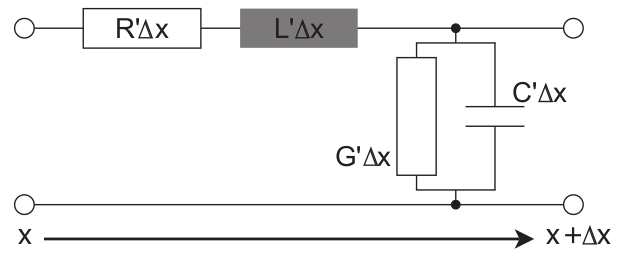
\includegraphics[width=0.8\textwidth]{img/ersatzschaltbild}
		\centering
		\caption{
			Ersatzschaltbild eines Leitungsabschnittes eines transversalelektromagnetischen Leiters. \cite{Anleitung}
		}
		\label{fig_ersatzschaltbild}
		\centering
	\end{figure}

	Aufstellen der Gleichungen für Maschen- und Knotenregel (vgl. \cite{Anleitung} ) führt zur Übertragungsfunktion:
	\begin{align}
		U(x) &= U_h \cdot e^{-\gamma x} + U_r \cdot e^{\gamma x}\\
		I(x) &= I_h \cdot e^{-\gamma x} - I_r \cdot e^{\gamma x}\\
		\text{mit} \quad \gamma \vcentcolon &= \sqrt{(R'+i \omega L')(G' +i \omega C')} = \alpha + i \beta
	\end{align}
	Dabei ist $\alpha $ der Dämpfungskoeffizient.

	\subsection{Leitungsabschluss}
	Wenn an einem Kabelende keine Reflexionen auftauchen sollen, muss der Reflexionskoeffizient verschwinden.
	Dieser ist definiert als:
	\begin{equation}
		r = \frac{Z_a-Z_L}{Z_a+Z_L} %TODO iirc war die Gleichung falsch (+- getauscht) und ist so richtig. ergibt auch Sinn.
	\end{equation}
	Dabei ist der  Leitungswiderstand
	\begin{equation}
		Z_L=\sqrt{\frac{L'}{C'}}.
	\end{equation}
	Der Abschlusswiderstand $Z_a$ soll also gleich zum Leitungswiderstand sein.

	Beim Reflexionskoeffizient entspricht $r=-1=1 \cdot e^{i\pi}$ einem Phasensprung von $\pi$.

	\subsection{Stehende Wellen}

	Stehende Wellen zeichnen sich dadurch aus, dass sie Knotenpunkte besitzen, an denen der Ausschlag stets Null ist und deren Position zeitlich konstant ist.
	Sie treten bei vollständiger Reflexion, also $| r | < 1	$, an eienr Barriere auf.

	Bei Betrachtung einer verlustlosen Leitungder Länge $l$, die an beiden Enden vollständig reflektiert, ergibt sich für die transmittierte Leistung die Airy-Funktion:

	\begin{align}
		P_t = \frac{|U_h|^2}{Z_L} \cdot \left( \frac{T}{1-R} \right) ^2 \cdot \frac{1}{1+F \sin^2 \left( \frac{\phi}{2} \right) } \\
		\text{mit dem Finesse-Faktor} \quad F= \frac{4R}{(1-R)^2} \\
		\text{und} \quad R = |r_1 ||r_2 |, \quad T= |t_1||t_2|,
	\end{align}
	wobei $t_{1,2}$ und $r_{1,2}$ die Reflexions- bzw. Transmissionskoeffizienten an den Leitungsenden sind.

	Diese wird maximal für
	\begin{equation}
	\sin ^2 \left( \frac{\phi}{2} \right) = 0 \Rightarrow 2k_nl -\varphi_1 - \varphi_2 = 2\pi n,
	\end{equation}
	wobei $\varphi_1, \varphi_2 $ die Phasensprünge an den beiden Enden der Leitung sind und $n \in \mathbb{Z}$.

	\subsection{Lecherleitung und Koaxialleitung}
	Bei der Lecherleitung verlaufen Feldlinien des elektromagnetischen Feldes weit außerhalb des Leiters und führen so zu erhöhtem Leitungswiderstand und erlauben ein Einkoppeln von Außen in die Übertragung.
	In einer Koaxialleitung wird dies dadurch, dass eine Leitung innerhalb der anderen verläuft minimiert.
	Der Vergleich ist in \cref{fig_lecherkoaxial} dargestellt.


	\begin{figure}[H]
        \centering
        \begin{subfigure}[b]{0.55\textwidth}
            \centering
            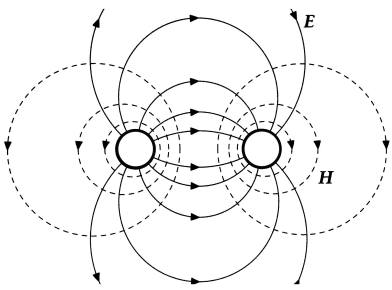
\includegraphics[width=\textwidth]{img/lecher}
            \caption{
							Lecherleitung
						}
            \label{fig_lecher}
        \end{subfigure}
        \hfill
        \begin{subfigure}[b]{0.40\textwidth}
            \centering
            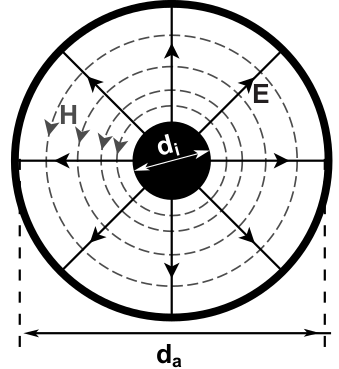
\includegraphics[width=\textwidth]{img/koaxial}
            \caption{
						Koaxialleitung
						}
            \label{fig_koaxial}
        \end{subfigure}

        \caption{Vergleich zwischen dem Verlauf der Feldlinien bei Lecher- und Koaxialleitung. \cite{Anleitung}}
				\label{fig_lecherkoaxial}
	\end{figure}


	\subsection{Mikrostreifenleitung}

	Wenn Mikrowellenleitungen auf Platinen verbaut werden sollen, ist die Koaxialleitung unpraktikabel.
	Hier kommt die Mikrostreifenleitung zum Einsatz, die, wie in \cref{fig_mikrostreifen} dargestellt, aus einem Leiter, der durch ein Dielektrikum von einer leitenden Fläche getrennt wird, besteht.
	Dies ist eine Kompromisslösung, da sie außerhalb verlaufende Feldlinien hat.

	\begin{figure}[H]
		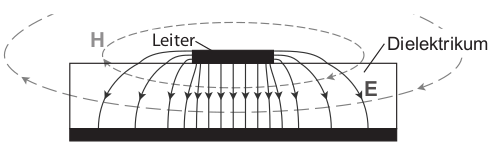
\includegraphics[width=0.8\textwidth]{img/mirkostreifen}
		\centering
		\caption{
			Verlauf der Feldlinien bei einer Mikrostreifenleitung. \cite{Anleitung}
		}
		\label{fig_mikrostreifen}
		\centering
	\end{figure}


	\subsection{Richtkoppler}


	\subsection{Zirkulator}


	\subsection{Isolator (Richtleitung)}


	\subsection{Detektordiode}

	\section{Methoden}
	% Bilder von der Website klauen
	% einer will Präsens

	\section{Ergebnisse und Diskussion}
	%TODO Unsicherheiten


	\subsection{Unsicherheiten}
	Alle Unsicherheiten werden nach GUM bestimmt und berechnet.
	Für diese Berechnungen wurde die Python Bibliothek \enquote{uncertainties} herangezogen, welche den Richtlinien des GUM folgt.

	\subsection{Kalibration der Detektordiode}
	% Allgemeine Beobachtungen
	% Einflüsse von veränderten Parametern auf Messung
	% Berechung nach Aufgabenstellung
	In \cref{fig_diode_kali} sind die aus verschiedenen Eingabeleistungen resultierenden Spannungen mit einer Exponentialfunktion \cref{eq_kali} angepasst worden.
	Die letzten drei Messpunkte wurden für den Fit ausgeschlossen, da die Diode dort in einen Sättigungsbereich kommt.

	\begin{equation}
		\label{eq_kali}
		U = A(e^{P/B}-C)
	\end{equation}

	\begin{figure}[H]
		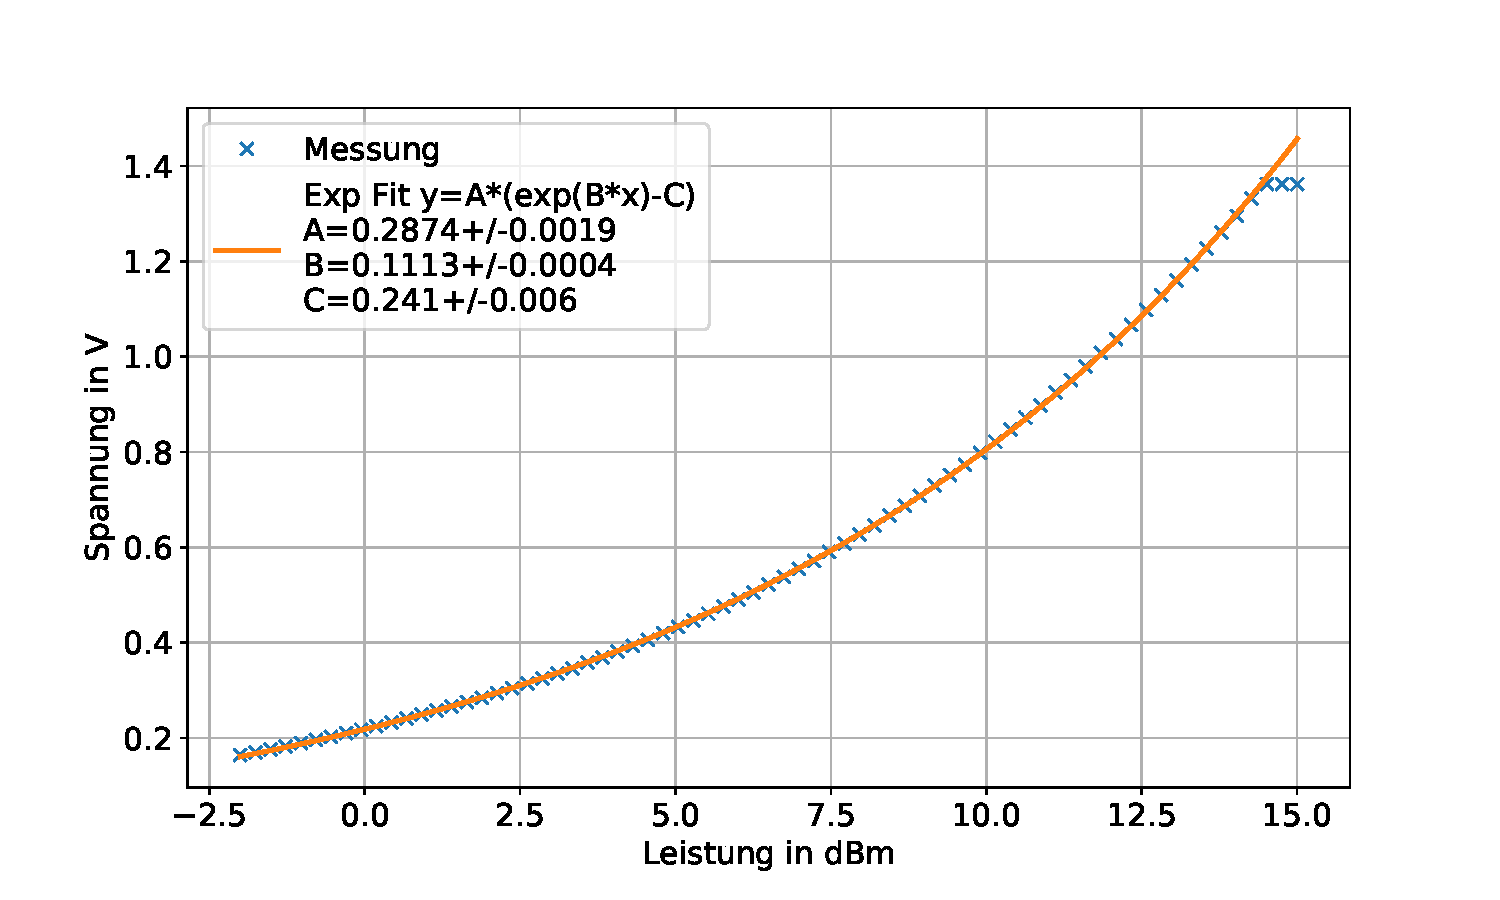
\includegraphics[width=0.8\textwidth]{img/diode-kali}
		\centering
		\caption{
			Am Multimeter gemessene Spannung bei verschiedenen Leistungen.
			Die Symbole sind größer als die Unsicherheiten.
		}
		\label{fig_diode_kali}
		\centering
	\end{figure}
	Mithilfe der Inversen Exponentialfunktion \label{eq_inv_kali} lassen sich im folgenden gemessen Spannungen in eine Leistung umrechnen.

	\begin{equation}
		\label{eq_inv_kali}
		P = B\log{(U/A+C)}
	\end{equation}
	\subsubsection*{Diskussion}
	% Bezug/Nutzen oder sonst was
	% auch hier die Hypothese wiederholen
	% keine Messwerte hier, nach manchen Menschen, zumindest "direkt" erstellte Diagramme net hier, auch wenn Lesbarkeit-bla


	\subsection{Isolator (Richtleitung)}
	In \cref{fig_isolator} ist die gemessene frequenzabhängige Dämpfung des Isolators in beide Richtungen abgebildet.
	Hierzu wurde die Spannung wie im vorherigen Abschnitt erläutert in eine Leistung umgerechnet.
	Die Dämpfung $\alpha$ ist
	\begin{equation}
		\alpha = 10 \cdot \log{(P_{\text{in}}/P_{\text{out}})} \cdot \si{dB}
	\end{equation}
  mit $P_\text{in}=\SI{10}{dBm}$.
	Und es folgt mit:
	\begin{equation}
		\alpha = 10 \cdot \log{\left(\frac{P_{\text{in}}}{P_{\text{out}}} \cdot \frac{1mW}{1mW}\right)} \cdot\si{dB}
	\end{equation}
	\begin{equation}
		\alpha = (P_\text{in} \text{[dBm]} - P_\text{out} \text{[dBm]} ) \cdot\si{dB}
	\end{equation}
	\begin{figure}[H]
		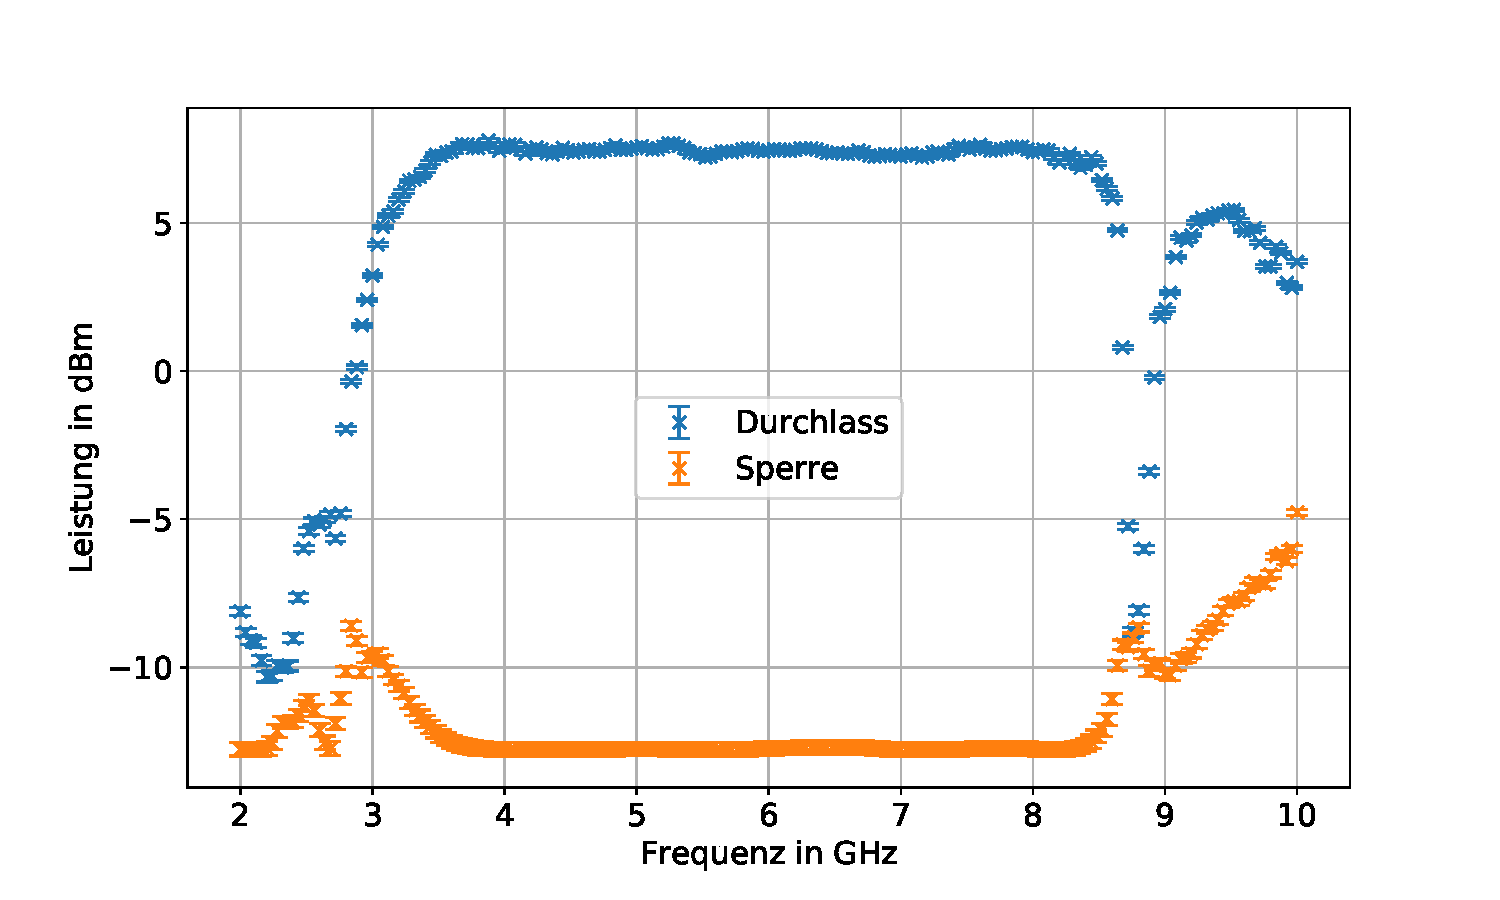
\includegraphics[width=0.8\textwidth]{img/isolator}
		\centering
		\caption{
		Durchlass- und Sperrdämpfung des Isolators in Abhängigkeit der Frequenz des Signals.
		}
		\label{fig_isolator}
		\centering
	\end{figure}
	\subsubsection*{Diskussion}
	%TODO Bandbreite Abschätzen und ggf. vergleichen mit Lit.

	\subsection{Richtkoppler}
	In analoger Weise erhält man auch die frequenzabhängigen Dämpfungen des Richtkopplers.
	Wobei $P_\text{in}$ wieder \SI{10}{dBm} ist.
	\begin{figure}[H]
		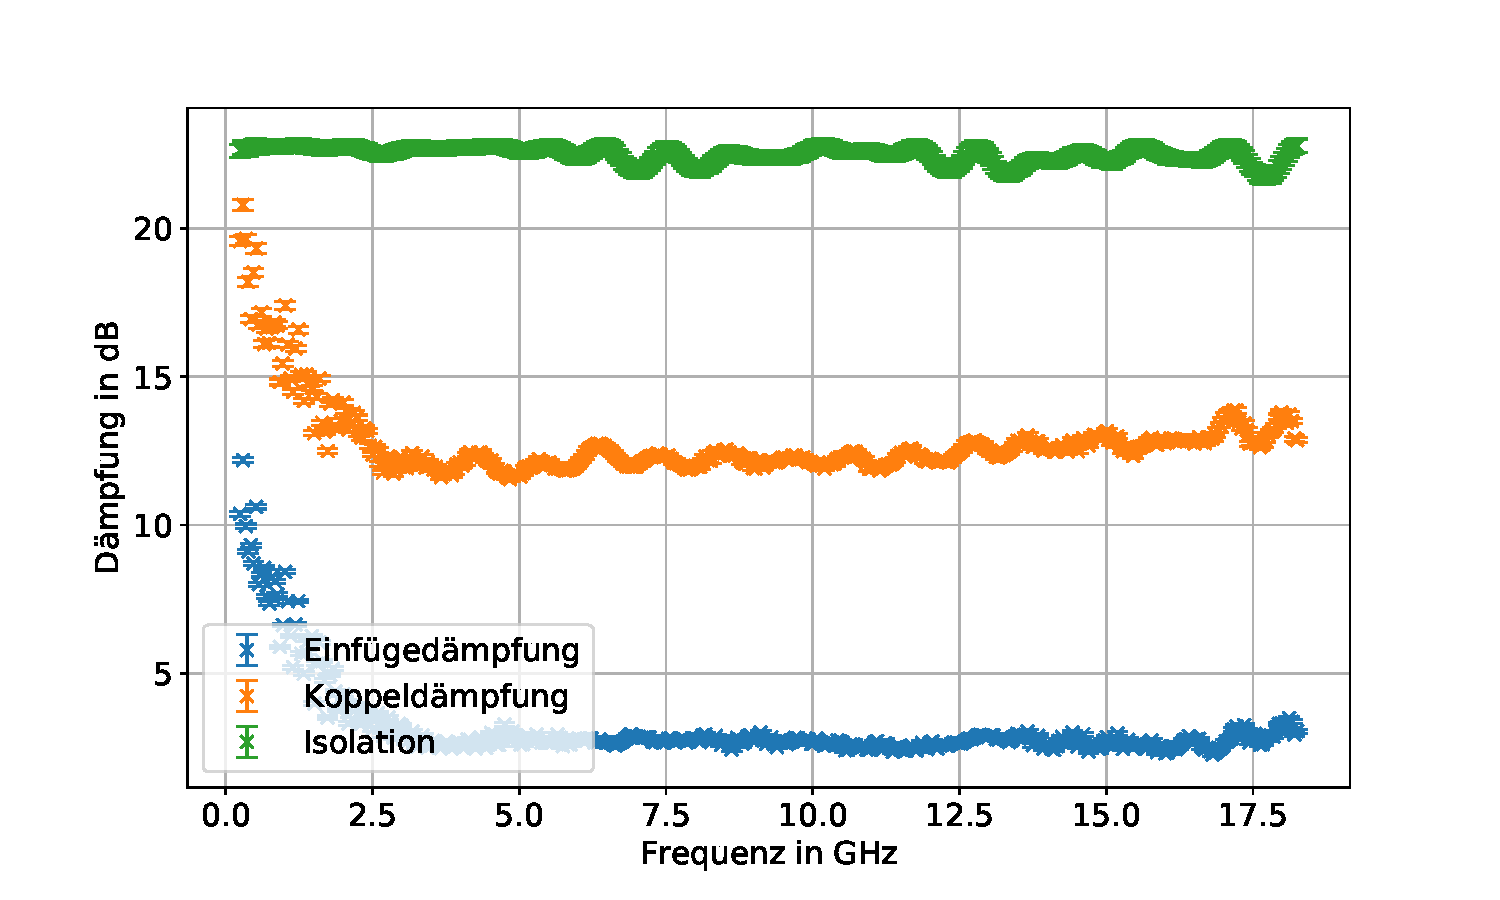
\includegraphics[width=0.8\textwidth]{img/richtkop}
		\centering
		\caption{
		Einfüge-, Koppel sowie Isolationsdämpfung des Richtkopplers in Abhängigkeit der Frequenz des Signals.
		}
		\label{fig_isolator}
		\centering
	\end{figure}
	\subsubsection*{Diskussion}

	\subsection{Zirkulator}
	\subsubsection*{Diskussion}

	\subsection{Stehende Wellen}
	\subsubsection*{Diskussion}

	\section{Schlussfolgerung}
	% Rückgriff auf Hypothese und drittes Nennen dieser

	% Quellen zitieren, Websiten mit Zugriffsdatum
	% Verweise auf das Laborbuch (sind erlaubt)
	% Tabelle + Bilder mit Beschriftung
	\printbibliography
\end{document}
